{ % Command scope

\newcommand{\INSTANCE}{I}
\newcommand{\STORAGE}{S}
\newcommand{\PROVIDER}{P}
\newcommand{\PROVIDERINSTANCES}{PI}
\newcommand{\LOCALSTORAGE}{LS}

\newcommand{\instancePrice}{p^I}
\newcommand{\ccu}{ccu}
\newcommand{\instanceTransferPriceIn}{p^{Iin}}
\newcommand{\instanceTransferPriceOut}{p^{Iout}}
\newcommand{\storageTransferPriceOut}{p^{Sout}}
\newcommand{\storageTransferPriceIn}{p^{Sin}}
\newcommand{\transferRate}{r}
\newcommand{\totalTasks}{A^{tot}}
\newcommand{\transferTime}{t^{net}}
\newcommand{\execTime}{t^x}
\newcommand{\dataSizeIn}{d^{in}}
\newcommand{\dataSizeOut}{d^{out}}
\newcommand{\requestPrice}{p^{R}}
\newcommand{\deadline}{t^D}
\newcommand{\instanceDeadline}{t^d}
\newcommand{\unitTime}{t^u}
\newcommand{\transferCost}{c^t}
\newcommand{\tasksPerDeadline}{a^d}
\newcommand{\timeQuantum}{t^q}
\newcommand{\tasksPerTimeQuantum}{a^q}
\newcommand{\providerMaxMachines}{n^{Pmax}}
\newcommand{\instanceMaxMachines}{n^{Imax}}

\newcommand{\NumberInstances}{N}
\newcommand{\TaskAssignment}{A}
\newcommand{\DataAssignment}{D}
\newcommand{\TailTaskHours}{R}
\newcommand{\HasTail}{H}

\chapter{Bag of tasks optimization}
\label{chap:bot} 
\lhead{Chapter \ref{chap:bot}. \emph{Bag of tasks optimization}}

   In this chapter we discuss optimization of scientific applications that may be represented as bag of uniform tasks. The chapter is organized as follows: after defining application model in Section~\ref{sec:bot:appmodel} and infrastructure model in Section~\ref{sec:bot:cloudmodel}, we formulate the problem using AMPL by specifying the variables, parameters, constraints and optimization goals in \ref{sec:bot:problem}. Section~\ref{sec:bot:results} presents the results obtained by applying the model to the scenarios involving multiple public and private clouds, overlapping computation and data transfers, and identifying special cases. Section~\ref{sec:bot:sensitivity} provides a sensitivity analysis of the model and show how such analysis can be useful for potential users or computing service resellers. Section~\ref{sec:bot:dynamic} shows estimation on how the model behaves if the task sizes are not uniform and change dynamically.

\section{Application model}
\label{sec:bot:appmodel}

  The goal of this optimization model is to minimize the cost of processing a given number of tasks on a hybrid cloud platform, as discussed in Section.~\ref{sec:bot:cloudmodel}. We assume that tasks are independent from each other, but they have identical computational cost and require a constant amount of data transfer.  
  
  We assume that for each task a certain amount of input data needs to be downloaded, and after it finishes, the output results need to be stored. In the case of data-intensive tasks, the transfers may contribute a significant amount of total task run time.

  The assumption of homogeneous tasks can be justified by the reason that there are many examples of scientific applications (e.g. scientific workflows or large parameter sweeps) that include a stage of a high number of parallel nearly identical tasks. Such examples can be found e.g. in typical scientific workflows executed using Pegasus Workflow Management system, where e.g. CyberShake or LIGO workflows have a parallel stage of nearly homogeneous tasks~\cite{Bharathi08}. Other examples are Wien2K and ASTRO workflows that consist of iteratively executed parallel stages comprising homogeneous tasks~\cite{Duan12}. Due to the high number of parallel branches, these stages accumulate the most significant computing time of the whole application, so optimization of the execution of this stage is crucial. Moreover, if the tasks are not ideally homogeneous, it is possible to approximate them using a uniform set of tasks with the mean computational cost and data sizes of the application tasks. Of course, in real execution the actual task performance may vary, so the solution obtained using our optimization method becomes only approximate of the best allocation, and the actual cost may be higher and deadline may be exceeded. In order to estimate the quality of this approximation, we evaluate the impact of dynamic task runtime and and non-uniform tasks in section~\ref{sec:bot:dynamic}. 



\section{Infrastructure model}
\label{sec:bot:cloudmodel}

Three types of cloud services are required to run scientific application on the cloud: virtual machines, storage and networking. Amazon S3 and Rackspace Cloud Files are good examples of storage providers, while Amazon EC2, Rackspace, GoGrid and ElasticHosts represent computational services. In addition, the optimization model proposed in this thesis includes a private cloud running on own hardware. Each cloud provider offers multiple types of virtual machine instances with different performance and price.

For each provider the number of running virtual machines may be limited.  This is mainly the case for private clouds that have a limited capacity, but also the public clouds often impose limits on the number of virtual machines. E.g. Amazon EC2 allows maximum of 20 instances and requires to request a special permission to increase that limit~\cite{AmazonEC2FAQ}. 

Most of cloud providers charge their users for each running virtual machine on an hourly basis. Some providers charge in 5-minute (i.e. CloudSigma) or 1-minute cycles (i.e. Google Compute Engine), but it is not widespread practice yet. Additionally, users are charged for remote data transfer while local transfer inside provider's cloud is usually free. These two aspects of pricing policies may have a significant impact on the cost of completing a scientific task.

Cloud services are characterized by their pricing and performance. Instance types are described by price per hour, relative performance and data transfer cost as presented in Table~\ref{table:intro:cloud:pricing}. To assess the relative performance of clouds it is possible to run application-specific benchmarks on all of them, or to use publicly available cloud benchmarking services, such as CloudHarmony~\cite{CloudHarmony}. CloudHarmony defines performance of cloud instances in the units named CloudHarmony Compute Units (CCU) as similar to Amazon EC2 Compute Unit (ECU), which are approximately equivalent to CPU capacity of a 1.0-1.2 GHz 2007 Opteron or 2007 Xeon processor. Storage platforms include fees for data transfer.

\begin{table}
  \centering
  \begin{tabular}{| l | r | r |}
    \hline
    \textbf{Instance type} & \textbf{Price per hour} & \textbf{Instance performance in CCU} \\ \hline
    \multicolumn{3}{|c|}{\textbf{Amazon Web Services (AWS) [US East]}}       \\ \hline
    m2.4xlarge        & \$2.400   & 27.25                                    \\ \hline
    m2.2xlarge        & \$1.200   & 14.89                                    \\ \hline
    linux.c1.xlarge   & \$0.680   & 8.78                                     \\ \hline
    m2.xlarge         & \$0.500   & 7.05                                     \\ \hline
    m1.xlarge         & \$0.680   & 5.15                                     \\ \hline
    m1.large          & \$0.340   & 4.08                                     \\ \hline
    c1.medium         & \$0.170   & 3.43                                     \\ \hline
    m1.small          & \$0.085   & 0.92                                     \\ \hline
    \multicolumn{3}{|c|}{\textbf{Rackspace Cloud [Dallas]}}                  \\ \hline
    rs-16gb           & \$0.960   & 4.95                                     \\ \hline
    rs-2gb            & \$0.120   & 4.94                                     \\ \hline  
    rs-1gb            & \$0.060   & 4.93                                     \\ \hline
    rs-4gb            & \$0.240   & 4.90                                     \\ \hline
    \multicolumn{3}{|c|}{\textbf{GoGrid [CA, US]}}                           \\ \hline
    gg-8gb            & \$1.520   & 23.2                                     \\ \hline
    gg-4gb            & \$0.760   & 9.28                                     \\ \hline
    gg-2gb            & \$0.380   & 4.87                                     \\ \hline
    gg-1gb            & \$0.190   & 4.42                                     \\ \hline
    \multicolumn{3}{|c|}{\textbf{ElasticHosts [UK]}}                         \\ \hline
    eh-8gb-20gh       & \$0.654   & 9.98                                     \\ \hline
    eh-4gb-8gh        & \$0.326   & 5.54                                     \\ \hline
    eh-2gb-4gh        & \$0.164   & 4.75                                     \\ \hline
    eh-1gb-2gh        & \$0.082   & 4.30                                     \\ \hline
    \multicolumn{3}{|c|}{\textbf{Hypothetical instance of private cloud}}    \\ \hline
    private           & \$0.000   & 1.00                                     \\ \hline
  \end{tabular}
  \caption{Example pricing and performance of cloud instances.}
  \label{table:intro:cloud:pricing}  
\end{table}


\section{Problem formulation}
\label{sec:bot:problem}

  To perform optimization of the total cost, Mixed Integer Non-Linear Problem (MINLP) is formulated and implemented in A Mathematical Programming Language (AMPL)~\cite{Fourer2002}.  As we shown in Chapter~\ref{chap:ampl}, AMPL requires to specify input data sets and variables to define the search space, as well as constraints and objective function to be optimized.

\subsection{Input data}
 
  The formulation requires the following input sets, which represent the cloud infrastructure model:
  \begin{itemize}
      \item $\STORAGE = \{s3, cloudfiles\}$ -- defines available cloud storage
      sites,
      \item $\PROVIDER = \{amazon, rackspace, \dotsc\}$ -- defines
      possible computing cloud providers,
      \item $\INSTANCE = \{m1.small, \dots, gg.1gb, \dotsc\}$ -- defines
      instance types,
      \item $\PROVIDERINSTANCES_{p} \subset \INSTANCE$ -- instances that
      belong to provider $\PROVIDER_p$,
      \item $\LOCALSTORAGE_{s} \subset \PROVIDER$ -- compute cloud providers
      that are local to storage platform $\STORAGE_s$.
  \end{itemize}        
    
  Each instance type $\INSTANCE_i$ is described by the following parameters:
  \begin{itemize}
      \item $\instancePrice_i$ -- fee in \$ for running instance $\INSTANCE_i$
      for one hour,
      \item $\ccu_i$ -- performance of instance in CloudHarmony Compute Units
      (CCU),
      \item $\instanceTransferPriceOut_i$ and $\instanceTransferPriceIn_i$ --
      price for non-local data transfer to and from the instance, in \$ per
      MiB.
  \end{itemize}

  Storage sites are characterized by:
  \begin{itemize}
      \item $\storageTransferPriceOut_s$ and $\storageTransferPriceIn_s$
      characterize price in \$ per MiB for non local data transfer.
  \end{itemize}

  Additionally, we need to provide data transfer rates in MiB per second between storage and instances by defining function $\transferRate_{i,s} > 0$ .

  We assume that the computation time of a task is known and constant, this also applies to input and output data size. We also assume that tasks are atomic (non divisible). Computation is characterized by the following parameters:
  \begin{itemize}
      \item $\totalTasks$ -- number of tasks,
      \item $\execTime$ -- execution time in hours of one task on 1 CCU
      machine,
      \item $\dataSizeIn$ and $\dataSizeOut$ -- data size for input and
      output of one task in MiB,
      \item $\requestPrice$ -- price per request for queuing service,
      \item $\deadline$ -- total time for completing all tasks in hours (deadline).
  \end{itemize} 

\subsection{Auxiliary parameters}

  The formulation of the problem requires a set of precomputed parameters which are derived from the main input parameters of the model. The relevant  parameters include:
  \begin{align}
      \transferTime_{i,s} &= \frac{\dataSizeIn+\dataSizeOut}{\transferRate_{i,s} \cdot 3600}  \\
      \label{bot:unitTime}\unitTime_{i,s} &= \frac{\execTime}{\ccu_i} + \transferTime_{i,s}  \\
      \transferCost_{i,s} &= (\dataSizeOut \cdot (\instanceTransferPriceOut_i + \storageTransferPriceIn_s) + \dataSizeIn \cdot (\storageTransferPriceOut_s+\instanceTransferPriceIn_i)) \\
      \label{bot:tasksPerDeadline}\tasksPerDeadline_{i,s} &= \lfloor\frac{\deadline}{\unitTime_{i,s}}\rfloor \\
      \timeQuantum_{i,s} &= \lceil \unitTime_{i,s} \rceil \\
      \tasksPerTimeQuantum_{i,s} &= \lfloor\frac{\timeQuantum_{i,s}}{\unitTime_{i,s}}\rfloor \\
      \label{bot:instanceDeadline}\instanceDeadline_{i,s} &= \lceil\lfloor\frac{\deadline}{\unitTime_{i,s}} \rfloor \cdot \unitTime_{i,s} \rceil
  \end{align}
  \begin{itemize}
      \item $\transferTime_{i,s}$ -- {\em transfer time}: time for data transfer between
      $\INSTANCE_i$ and $\STORAGE_s$,
      \item $\unitTime_{i,s}$ -- {\em unit time}: time for processing a task
      on instance $\INSTANCE_i$ using storage $\STORAGE_s$ that includes computing and
      data transfer time (in hours),
      \item $\transferCost_{i,s}$ -- cost of data transfer between instance
      $\INSTANCE_i$ and storage $\STORAGE_s$,
      \item $\tasksPerDeadline_{i,s}$ -- number of tasks that can be done on
      one instance $\INSTANCE_i$ when using storage $\STORAGE_s$ running for $\deadline$ hours,
      \item $\timeQuantum_{i,s}$ -- {\em time quantum}: minimal increase of
      instance running time that is sufficient to increase the number of
      processed tasks, rounded up to full hour,
      \item $\tasksPerTimeQuantum_{i,s}$ -- number of tasks that can be done
      in $\timeQuantum_{i,s}$ hours,
      \item $\instanceDeadline_{i,s}$ -- {\em instance deadline}: number of
      hours that can be effectively used for computation.
  \end{itemize}

\subsection{Variables}
\label{sec:bot:varialbes}
  Variables that will be optimized and define the solution space are listed below:
  \begin{itemize}
      \item $\NumberInstances_i$ -- number of instances of type $\INSTANCE_i$
      to be deployed,
      \item $\TaskAssignment_i$ -- number of tasks to be processed on
      instances of type $\INSTANCE_i$,
      \item $\DataAssignment_s$ -- $1$ iif $\STORAGE_s$ is used, otherwise $0$; only one storage may be used,
      \item $\TailTaskHours_i$ -- number of remainder (tail) hours for
      instance $\INSTANCE_i$,
      \item $\HasTail_i$ -- $1$ iif $\TailTaskHours_i \neq 0$, otherwise $0$.
  \end{itemize}


  Fig.~\ref{fig:bot:policy} illustrates how the tasks are assigned to multiple running instances. The tasks are atomic and there is no checkpointing or preemption. Even though all the tasks have the same computational cost, their total processing time depends on performance of the VM type and data transfer rate. Moreover, the users are charged for the runtime of each VM rounded up to full hours. In our model the tasks are assigned to the instances in the following way. First, in the process of optimization $\TaskAssignment_i$ tasks are assigned to the instance $\INSTANCE_i$. This gives $\NumberInstances_i$  instances of type $\INSTANCE_i$ running for $\instanceDeadline_{i,s}$ hours. Remaining tasks are assigned to an additional instance running for $\TailTaskHours_i$ hours. We will refer to them as tail hours.

  \begin{figure}[tb] 
     \centering
     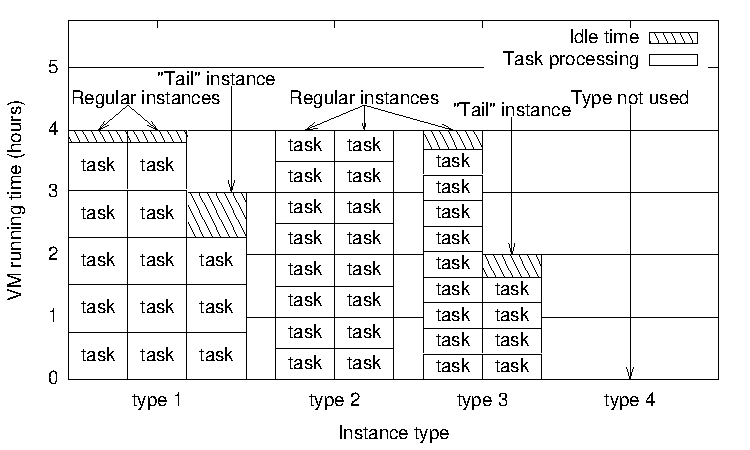
\includegraphics[width=0.7\columnwidth]{BagOfTasks/scheduling_policy.pdf}
     \caption{\label{fig:bot:policy}Task scheduling policy}
  \end{figure}
    

  In order to enforce provider's instance limit, $\HasTail_i$ is introduced which indicates if $\INSTANCE_i$ has any tail hours. E.g. in Fig.~\ref{fig:bot:policy} instances of type 1 have 3 tail hours, and instances of type 2 have no tail hours.


\subsection{Formulation of constraints and objectives}

  Cost of running a single task which includes the cost of VM instance time required for data transfer and task computing time, together with data transfer costs and request cost, can be described as: 

  \begin{align*}
      \left(\transferTime + \unitTime\right) \cdot \instancePrice + \\
      \dataSizeIn \cdot \left(\storageTransferPriceOut + \instanceTransferPriceIn\right) + \\
      \dataSizeOut \cdot \left(\instanceTransferPriceOut + \storageTransferPriceIn\right) + \\
      \requestPrice
  \end{align*}

  The objective function represents the total cost of running multiple tasks of the application on the cloud infrastructure and it is defined as:

  \begin{align}    
      \underset{\text{total cost}}{\text{minimize}} \sum \limits_{i \in \INSTANCE}  ( & 
                   (\sum\limits_{s \in \STORAGE} \DataAssignment_s\cdot\instanceDeadline_{i,s}\cdot\NumberInstances_i + \TailTaskHours_i) \cdot \instancePrice_i  
                    + \TaskAssignment_i\cdot(\requestPrice + \sum\limits_{s \in \STORAGE} \DataAssignment_s \cdot \transferCost_{i,s})
                 )
  \end{align}
  
  subject to the constraints:
  \nopagebreak 
  \begin{align}
     \label{bot:cSolutionConstraintsBegin}\mathop\forall\limits_{i \in \INSTANCE} & \TaskAssignment_i \in \mathbb{Z} \land 0 \leq \TaskAssignment_i \leq \totalTasks  \\
     \mathop\forall\limits_{s \in \STORAGE}  & \DataAssignment_s \in \{0, 1\} \\ 
     \mathop\forall\limits_{i \in \INSTANCE} & \NumberInstances_i \in \mathbb{Z} \land 0 \leq \NumberInstances_i \leq \instanceMaxMachines_i \\
     \mathop\forall\limits_{i \in \INSTANCE} & \TailTaskHours_i \in \mathbb{Z} \land 0 \leq \TailTaskHours_i \leq \deadline - 1 \\
     \label{bot:cSolutionConstraintsEnd}\mathop\forall\limits_{i \in \INSTANCE} & \HasTail_i \in \{0, 1\} \\
     \label{bot:cTaskAssignmentBounds}\mathop\forall\limits_{i \in \INSTANCE}
          & \TaskAssignment_i \geq \sum_{s \in \STORAGE} (\NumberInstances_i \cdot
          \tasksPerDeadline_{i,s}) \cdot \DataAssignment_s
          \\
      \label{bot:cTaskAssignmentBounds2}\mathop\forall\limits_{i \in \INSTANCE}
          & \TaskAssignment_i \leq  \sum_{s \in \STORAGE} (\NumberInstances_i \cdot
          \tasksPerDeadline_{i,s} + \max(\tasksPerDeadline_{i,s} - 1, 0)) \cdot
          \DataAssignment_s\\
     \label{bot:cTailTasksHoursBounds}\mathop\forall\limits_{i \in \INSTANCE}
          & \TailTaskHours_i \geq \sum_{s \in \STORAGE} (\TaskAssignment_i - \NumberInstances_i \cdot
          \tasksPerDeadline_{i,s}) \cdot \unitTime_{i,s} \cdot \DataAssignment_s
          \\ 
     \label{bot:cTailTasksHoursBounds2}\mathop\forall\limits_{i \in \INSTANCE}
          & \TailTaskHours_i  \leq \sum_{s \in \STORAGE} (\TaskAssignment_i -
          \NumberInstances_i \cdot \tasksPerDeadline_{i,s} +
          \tasksPerTimeQuantum_{i,s}) \cdot \unitTime_{i,s} \cdot
          \DataAssignment_s\\ 
     \label{bot:cSumTasks}& \sum\limits_{i \in \INSTANCE} \TaskAssignment_i = \totalTasks \\
     \label{bot:cData}& \sum\limits_{s \in \STORAGE} \DataAssignment_s = 1 \\ 
     \label{bot:cSetHasTailBounds}\mathop\forall\limits_{i \in \INSTANCE} &
     \HasTail_i \leq \TailTaskHours_i \leq \max(\deadline-1,0)\cdot\HasTail_i
     \\ \label{bot:cMaxMachines}\mathop\forall\limits_{p \in \PROVIDER} & \sum_{i \in \PROVIDERINSTANCES_p} (\HasTail_i + \NumberInstances_i) \leq \providerMaxMachines_p
  \end{align}

  Interpretation of the constraints is the following:
  \begin{itemize}
      \item(\ref{bot:cSolutionConstraintsBegin}) to
      (\ref{bot:cSolutionConstraintsEnd}) define weak constraints for a solution, i.e. they are to ensure that the required variables have the appropriate integer or binary values,
      \item(\ref{bot:cTaskAssignmentBounds}) and (\ref{bot:cTaskAssignmentBounds2}) ensure that number of instances is adequate to number of assigned tasks; for chosen storage $\DataAssignment_s$
      \begin{align*}
          \NumberInstances_i \cdot \tasksPerDeadline_{i,s} \leq \TaskAssignment_i \leq \NumberInstances_i \cdot \tasksPerDeadline_{i,s} + \max\left(\tasksPerDeadline_{i,s} - 1, 0\right)
      \end{align*} where the lower bound is given by full allocation of $\NumberInstances_i$ machines and the upper bound includes a fully allocated tail machine,
      \item(\ref{bot:cTailTasksHoursBounds}) and (\ref{bot:cTailTasksHoursBounds2})
      ensure that number of tail hours is adequate to number of remaining
      tasks, implement $\TailTaskHours_i = \ceil*{\left(\TaskAssignment_i - \NumberInstances_i \cdot \tasksPerDeadline_{i,s}\right) \cdot \unitTime_{i_s}}$,
      \item(\ref{bot:cSumTasks}) ensures that all tasks are processed,
      \item(\ref{bot:cData}) ensures that only one storage site is selected,
      \item(\ref{bot:cSetHasTailBounds}) ensures that $\TailTaskHours_i$ has proper value,
      implements $\HasTail_i = \left\{\begin{array}{cc} 1, & \TailTaskHours_i\; >\; 0 \\ 0, & \TailTaskHours_i\; =\; 0 \end{array}\right.$,
      \item(\ref{bot:cMaxMachines}) enforces providers' instance limits. 
  \end{itemize}

\subsection{Solver choice}

  Defining the problem in AMPL enables to choose among a wide range of solvers that can be used as backend. The problem itself is MINLP, but can be reduced to Integer Linear Programming (ILP) problem. The nonlinear part of problem comes from storage choice, so by fixing storage provider and running optimization procedure for each storage separately the optimal solution is found.

  Initially {Bonmin}~\cite{Bonami2008} solver was used, but after the model was fully implemented and subject to more tests, it appeared that CBC~\cite{cbc-solver} solver performs better with default options. This results from the fact that {Bonmin} is a solver designed to solve MINLP problems and uses various heuristics, while CBC uses a branch and bound algorithm tuned for ILP. As the problem is linear and convex, CBC finds global optimum. The model was optimized so that it should give acceptable results in $\sim$0.10 seconds \footnote{As measured on quad-core Intel i5 machine.}. 

\section{Experiments and results}
\label{sec:bot:results}
    
  To evaluate the model, we first run the optimization process for two scenarios with a private cloud and (1) infinite public clouds (Section~\ref{sec:bot:private-infinite}) and (2) finite public clouds (Section~\ref{sec:bot:private-finite}). We also evaluated the effect of possible overlapping of computations and data transfers in Section~\ref{sec:bot:overlapping}. When testing the model under various input parameters, we identified interesting special cases described in Section~\ref{sec:bot:special}. Finally, we discuss a sensitivity analysis, its implications and potential usage in Section~\ref{sec:bot:sensitivity}.
    
  Data intensive tasks that require relatively large amount of data for short computing time (we assumed 512 MiB of input and 512 MiB of output) and compute intensive tasks that require relatively small amount of data (we assumed 0.25 MiB of input and 0.25 MiB of output). Each case consists of 20,000 tasks, each of them requires 0.1 hour of computing time on a VM with performance of 1 CCU. Two scenarios with infinite and finite public clouds were considered, where as the costs and performance of public clouds we used the data from CloudHarmony benchmarks. This dataset gives the data of 4 compute cloud providers (Amazon EC2, Rackspace, ElasticHosts and GoGrid) and 2 storage providers (Amazon S3 and Rackspace Cloud Files), giving the instance prices between \$0.06 and \$2.40 per hour and performance between 0.92 and 27.4 CCU (see Table~\ref{table:intro:cloud:pricing}). The pricing model assumes that the private cloud instances have the performance of 1 CCU and \$0 cost.  For each scenario the deadline parameter ranges between 5 and 100 hours.  Since only two storage providers (S3 and Cloud Files) were considered, the solver is run separately for these two parameters.
    
\subsection{Private + infinite public clouds}
\label{sec:bot:private-infinite} 
  This scenario assumes that the private cloud can run a maximum of 10 instances, while the public clouds have unlimited capacity. The results for tasks that require small amount of data are shown in Fig.~\ref{fig:bot:small-infinite}. As the deadline is extended, the total cost linearly drops as expected. As many tasks as possible are run on the private cloud, and for all the remaining tasks the instance type with best price to performance ratio is selected.
    
  This situation changes as data size grows (Fig.~\ref{fig:bot:large-infinite}) -- for data intensive tasks the total cost is nearly constant as all the work is done on a public cloud. This results from the fact that data transfer cost to and from the private cloud is higher than the cost of running instances on public cloud. In our case it turns out that the lowest cost can be achieved when using Cloud Files storage from Rackspace, since in our dataset the best instance type in terms of price to performance was available at Rackspace. 
        
  \begin{figure}[tb] 
     \centering
     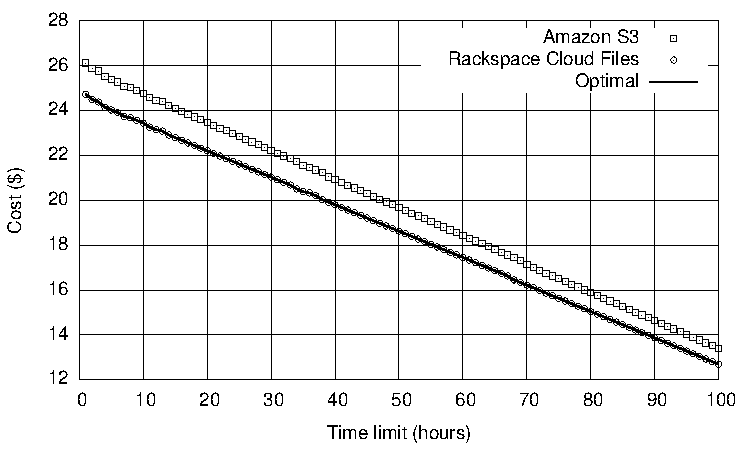
\includegraphics[width=0.7\columnwidth]{BagOfTasks/graph-small-infinite.pdf}
     \caption{Small data processed on infinite public cloud\label{fig:bot:small-infinite}}
     
  \end{figure}

  \begin{figure}[tb] 
     \centering
     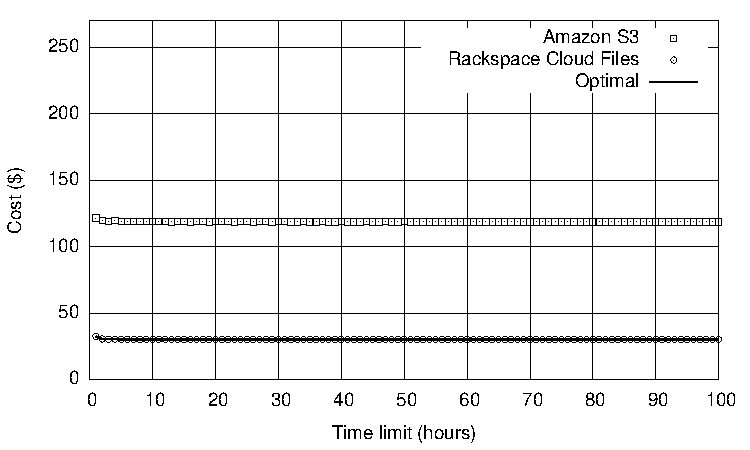
\includegraphics[width=0.7\columnwidth]{BagOfTasks/graph-large-infinite.pdf}
     \caption{Large data processed on infinite public cloud\label{fig:bot:large-infinite}}
  \end{figure}        
    
\subsection{Private + finite public clouds}
\label{sec:bot:private-finite}
    
  If assumption that public clouds are limited is made, situation is not so straightforward (See Fig.~\ref{fig:bot:small-finite} and~\ref{fig:bot:large-finite}). For relatively long deadlines, a single cloud platform for both VMs and storage can be used, which means that the data transfer is free. As the deadline shortens we first observe a linear cost increase. At the point when the selected cloud platform reaches its VM limit, additional clouds need to be used, so we need to begin paying for the data transfer. Therefore the cost begins to increase more rapidly.
  
  \begin{figure}[tb]
     \centering
     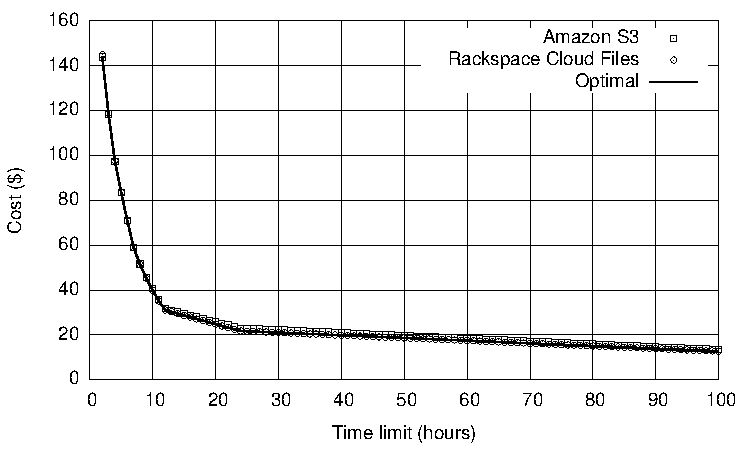
\includegraphics[width=0.7\columnwidth]{BagOfTasks/graph-small-finite.pdf}
     \caption{Small data processed on finite public
     cloud\label{fig:bot:small-finite}}
  \end{figure}

    
  This effect is very significant in the case of data intensive tasks (Fig.~\ref{fig:bot:large-finite}) as the cost growth may become very steep. For example, in our tests the task processing cost in 28 hours was \$157.39, in 30 hours it was \$131.14 and in 34 hours it was only \$30.26. For longer deadlines there was no further decrease. We can also observe that for longer deadlines the Cloud Files storage provider is less expensive for the same reason as it was in Fig.~\ref{fig:bot:large-infinite}. Shorter deadlines, however, require to run more powerful instances from other clouds (Amazon EC2), thus it becomes more economical to use its local S3 storage.
    
  \begin{figure}[tb]
     \centering
     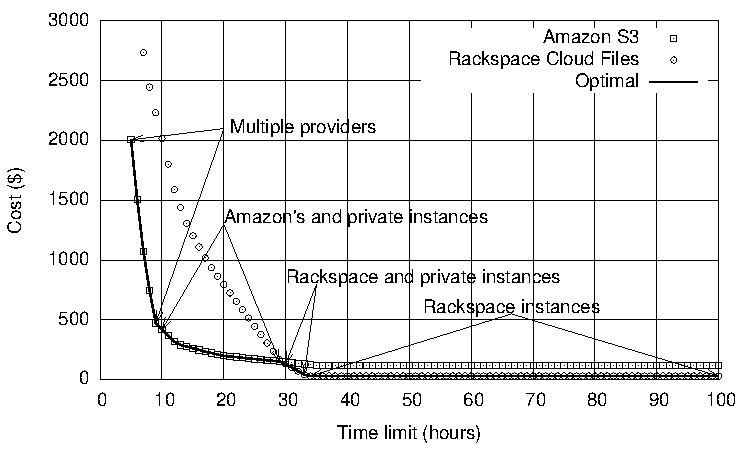
\includegraphics[width=0.7\columnwidth]{BagOfTasks/graph-large-finite.pdf}
     \caption{Large data processed on finite public
     cloud\label{fig:bot:large-finite}}
  \end{figure}  
  
\subsection{Overlapping computation and data transfers}
\label{sec:bot:overlapping}
  
  In the model we assumed that computation and data transfers are not overlapping. To achieve parallelism of these two processes, the model needs to be modified in the following way. The total task computation time is maximum of task execution and data transfer time. Additionally, input for the first task and output of the last task must be transferred sequentially. Equations \ref{bot:unitTime}, \ref{bot:tasksPerDeadline} and \ref{bot:instanceDeadline} are updated for this case as follows:
  
  \begin{align}
      \unitTime_{i,s} &= \max(\frac{\execTime}{\ccu_i}, \transferTime_{i,s})  \\    
      \tasksPerDeadline_{i,s} &= \lfloor\frac{(\deadline - \transferTime_{i,s})}{\unitTime_{i,s}}\rfloor \\         
      \instanceDeadline_{i,s} &= \lceil\lfloor\frac{(\deadline - \transferTime_{i,s})}{\unitTime_{i,s}} \rfloor \cdot \unitTime_{i,s} \rceil            
  \end{align}
  
  Fig.~\ref{fig:bot:large-finite-overlap} shows results for the same experiment as in Section~\ref{sec:bot:private-finite} and Fig.~\ref{fig:bot:large-finite}, but with computing and transfers overlapping. Overlapping reduces total cost as time required for task processing is significantly lower.  This is especially true for shorter deadlines when multiple clouds are used, as transfer rates are lower between different clouds comparing to one provider infrastructure.
  
  \begin{figure}[tb]
     \centering
     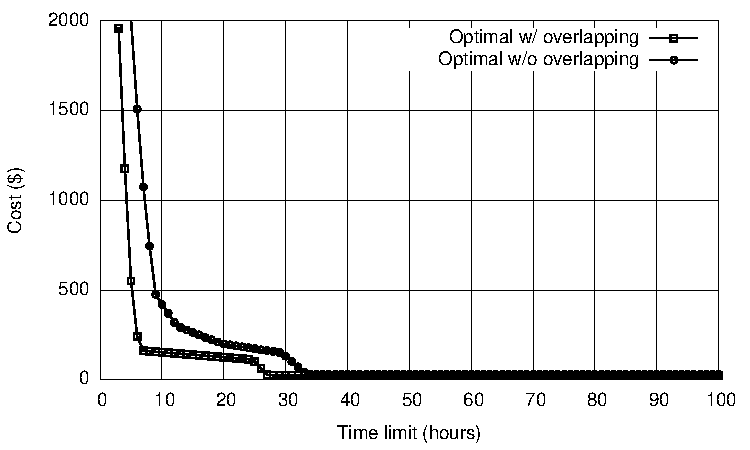
\includegraphics[width=0.7\columnwidth]{BagOfTasks/overlap.pdf}
     \caption{Large data processed on finite public cloud with overlapping computation and data transfer\label{fig:bot:large-finite-overlap}}
  \end{figure}  

\subsection{Identifying special cases}
\label{sec:bot:special}
  
  Running a test case with very large tasks which cannot be completed within one hour on largest available instance revealed an interesting model behavior. Results are shown on Fig.~\ref{fig:bot:special-case-results}. Local minima may occur for certain deadlines thus cost does not increase monotonically with decrease of deadline. This is a consequence of our task scheduling policy, as explained in Section~\ref{sec:bot:varialbes}. In the case of large tasks, the schedule for deadline of 9 hours  as seen in Fig.~\ref{fig:bot:special-case-009-cf} costs less than for deadline of 10 hours as in Fig.~\ref{fig:bot:special-case-010-cf}. In the first case the total number of VM-hours of the \emph{gg-8mb} instance is equal to 56, but in the case of deadline of 10 hours the total number is 58, which results in higher cost. This is the result of the policy, which tries to keep VMs running time as close to the deadline as possible. Such policy is based on general observation, that for a given budget it is usually more economical to start less VMs for longer time than to start more VMs for shorter time. However, there are rare cases when such policy may lead to non-optimal solutions. It should be noted, that the solution of the model returned by the solver in this case is optimal, but it is the model itself that does not allow to find the minimum cost.
  
  Moreover, for longer deadlines the cost is a step function -- e.g. the cost for deadline of 18 hours is the same as for 14 hours. These two observations suggest that the model could be modified in such a way that the deadline is also a variable with upper bound constraint. Similar result can be achieved in a simple way by solving the current model for multiple deadlines in the neighborhood of the desired deadline and by selecting the best solution.  
  
  \begin{figure}[tb]
     \centering 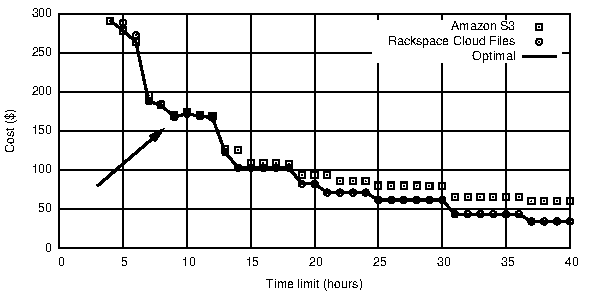
\includegraphics[width=0.7\columnwidth]{BagOfTasks/special-case-results.pdf}
     \caption{Special case with local minimum for deadline 9
     \label{fig:bot:special-case-results}}
  \end{figure}

  \begin{figure}[tb]
     \centering  
     \begin{subfigure}[b]{0.7\textwidth}
       \centering       
       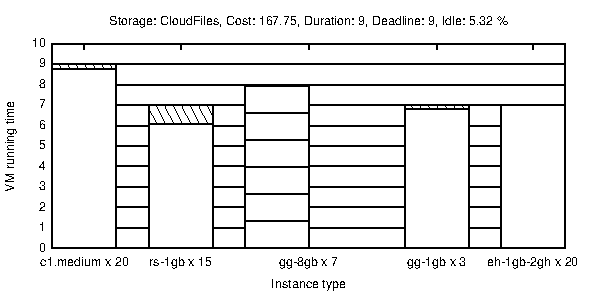
\includegraphics[width=\textwidth]{BagOfTasks/special-case-009-cf.pdf}
       \caption{Deadline = 9 hours}
       \label{fig:bot:special-case-009-cf}
     \end{subfigure}
     \begin{subfigure}[b]{0.7\textwidth}
       \centering       
       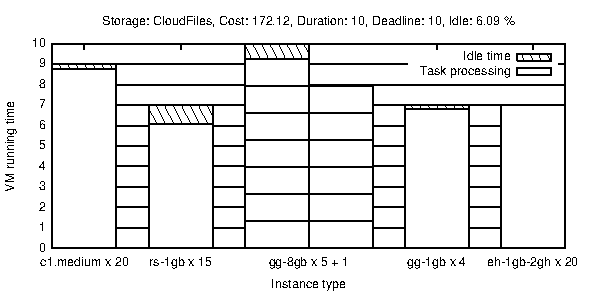
\includegraphics[width=\textwidth]{BagOfTasks/special-case-010-cf.pdf}
       \caption{Deadline = 10 hours}
       \label{fig:bot:special-case-010-cf}
     \end{subfigure}
     \caption{Task schedule for the identified special case}
  \end{figure}
    
\section{Sensitivity analysis}
\label{sec:bot:sensitivity}
    
  \begin{figure*}[tb]
     \centering 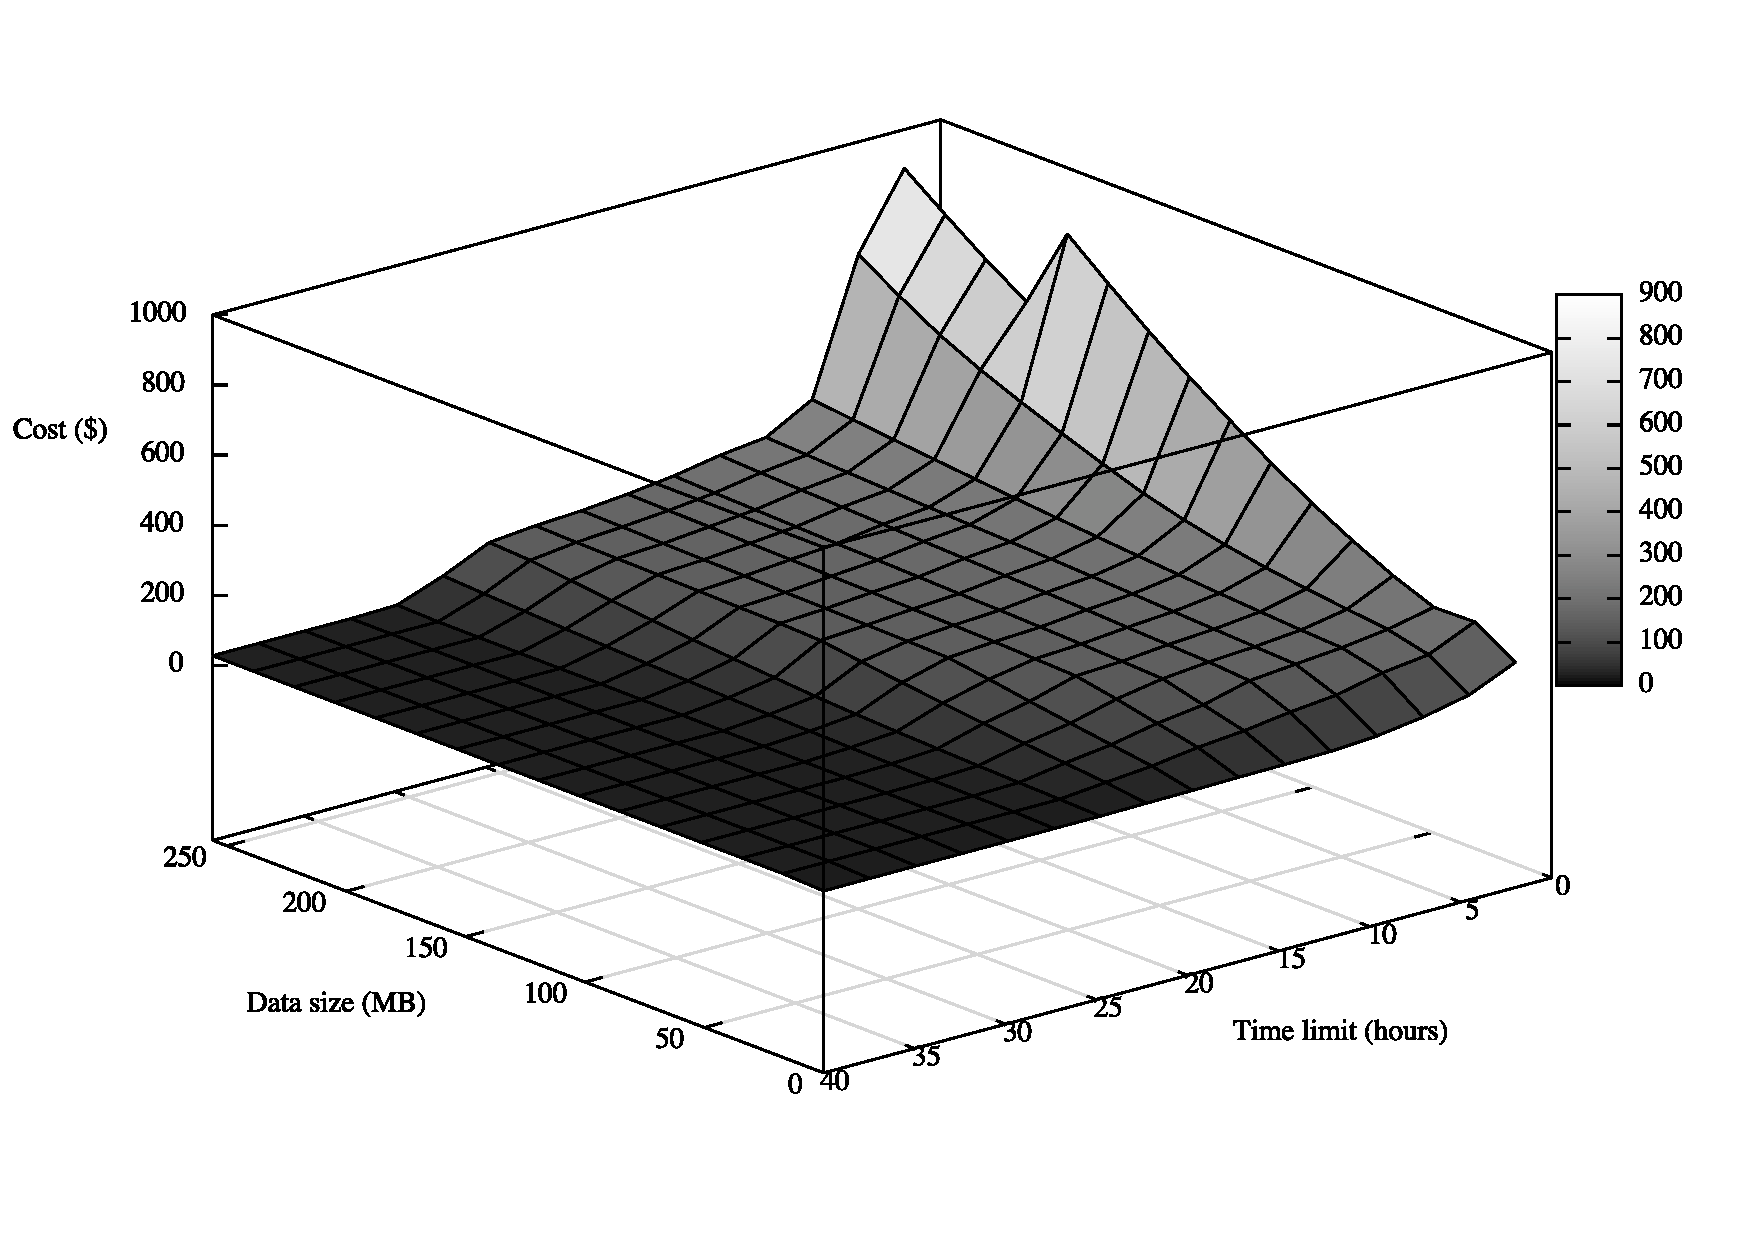
\includegraphics[width=0.7\textwidth]{BagOfTasks/sensitivity-surface}
     \caption{Optimal cost for a wide range of deadline constraints and data
     sizes.\label{fig:bot:sensitivity-surface}}
  \end{figure*} 
  
  In order to better assess how the model behaves in response to the changing
  constraints and for varying input parameters, I performed a sensitivity
  analysis by sampling a large parameter space.
  Fig. \ref{fig:bot:sensitivity-surface} shows the solutions obtained for deadlines
  ranging from 2 to 40 hours and for input and output data sizes ranging from
  0 to 256 MiB. As it can be seen in the plot, for all data sizes the cost
  increases monotonically with the decrease of the deadline, which confirms
  that no anomalies are observed. The same data can be also observed as
  animated plot available as on-line supplement\footnote{See also
  \url{http://youtu.be/FWjgMwLdZW4}}.
  
  \begin{figure}[tb]
     \centering 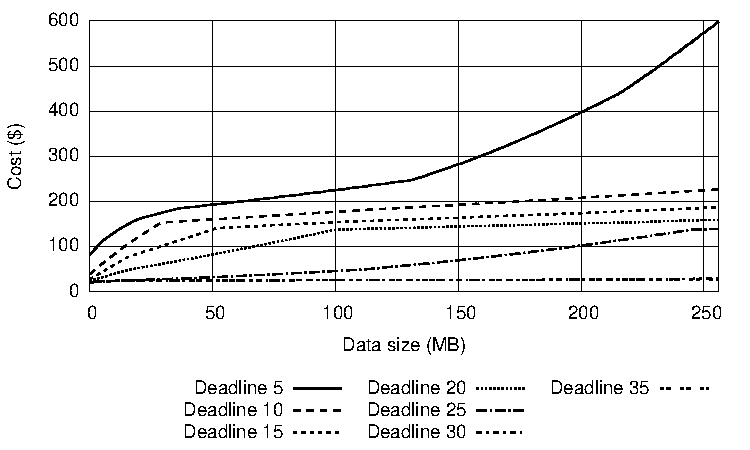
\includegraphics[width=0.7\columnwidth]{BagOfTasks/cost_vs_data_size}
     \caption{Cost as a function of data size for different
     deadlines.\label{fig:bot:cost_vs_data_size}}
  \end{figure} 
  
  Fig.~\ref{fig:bot:cost_vs_data_size} presents these results from a perspective
  where each curve shows how the cost depends on data size for varying
  deadlines.
  
  \begin{figure}[tb]
     \centering 
     \begin{subfigure}[b]{0.7\textwidth}
       \centering       
       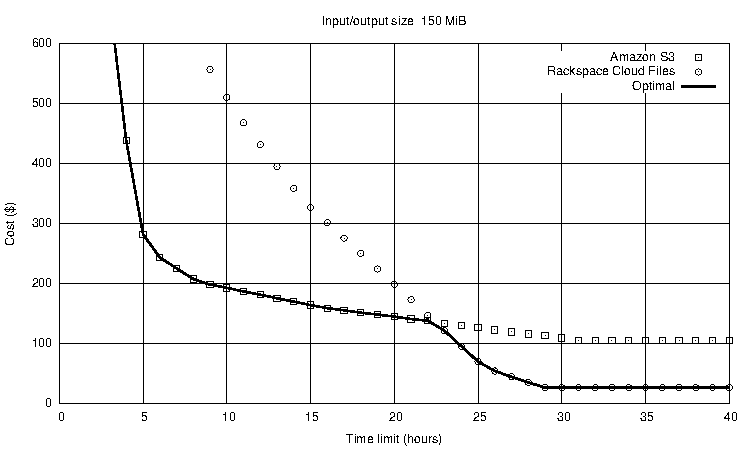
\includegraphics[width=\textwidth]{BagOfTasks/deadline-cost-150}
       \caption{Cost as a function of deadline}
     \end{subfigure}     
     \begin{subfigure}[b]{0.7\textwidth}
       \centering       
       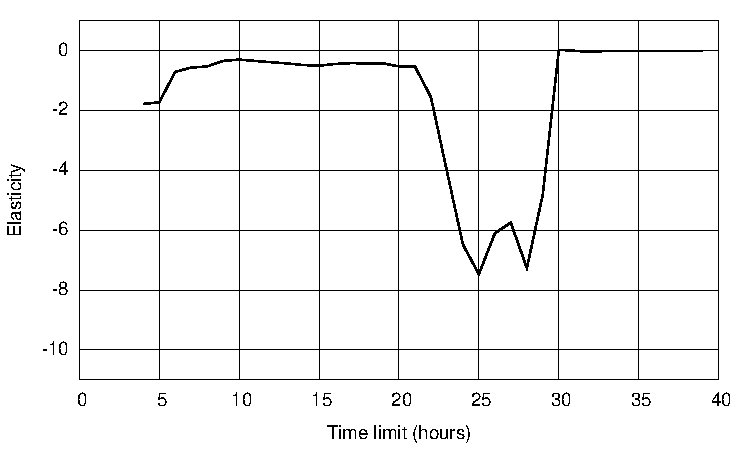
\includegraphics[width=\textwidth]{BagOfTasks/deadline-elasticity-150}
       \caption{Elasticity of cost versus deadline}
     \end{subfigure}     
     \caption{Sensitivity of costs in response to changes in deadline}
     \label{fig:bot:elasticity}
  \end{figure} 
  % 
  One of the questions that our model can help answer is how the changes in
  cost are sensitive to the changes of deadline. Fig.~\ref{fig:bot:elasticity} shows
  the cost function as well as corresponding elasticity, which is computed as:
  $E f(x) = \frac{x}{f(x)} f'(x)$, where in this case $f$ is cost and $x$ is
  deadline. Elasticity gives the information on what is the percentage change
  of cost in response to the percentage change of deadline. The function has
  negative values, since the cost decreases with the increase of deadline. It
  is interesting to see in which ranges the elasticity has larger absolute
  value, which corresponds to more steep cost function. Here we can see that
  the elasticity grows for short deadlines and close to the deadline of 25
  hours, which is the point where the solution cannot use only the VM instances
  from most cost-effective clouds and requires more expensive ones to meet the
  deadline.
  
  Identifying such ranges with high absolute value of elasticity is important
  for potential users of the cloud system, including researchers (end users) or
  resellers (brokers). The end user can for example observe that changing the
  deadline from 40 to 30 hours or even from 20 to 10 hours will not incur much
  additional cost. However, changing the deadline from 30 to 20 hours is very
  costly, so it should be avoided. On the other hand, the situation looks
  different from the perspective of a reseller, who buys cloud resources from
  providers and offers them to end-users in order to make profit. The reseller
  can for example offer to compute the given set of tasks in 20 hours for \$150
  with minimal profit, but it can also offer to complete the same set of tasks
  in 30 hours for \$50. Such price can seem attractive to the end user who pays
  1/3 of the price for increasing the deadline by 50\%, but it is in fact very
  beneficial for the reseller, whose profit reaches 100\%. Such cost analysis
  is an important aspect of planning large computing experiments on cloud
  infrastructures.

\section{Impact of dynamic environment}
\label{sec:bot:dynamic}
    
  As stated in section~\ref{sec:bot:appmodel}, we assume that execution time,
  transfer rate and data access time for all the tasks are constant. However,
  in real environments the actual runtime of tasks will vary. The goal of the
  following simulation experiment was to estimate the impact of this runtime
  variation on the quality of results obtained using our optimization model.
  
  For all the task assignment solutions presented in Fig.~\ref{fig:bot:sensitivity-surface} 
  we add runtime variations to the task runtimes in the following way. For each task
  we generate a random error in the range from $-v$ to $v$ using uniform distribution,
  where $v$ is the runtime variation range. We tested values of $v=10\%, 20\%, 30\%, 40\%, 50\%$. 
  Such modified task runtimes are then used to calculate the actual runtime and cost of 
  VM. Due to variation of task runtimes, it is possible that some computations may not 
  finish before the deadline (time overrun) and that the cost of additional VM-hours
  may need to be paid (cost overrun).

  We assume that task size variations include also
  variations of data transfer time. We don't take into account variations of
  data transfer costs, since the transfer costs for each task depend linearly
  on data size, so the aggregated impact of positive and negative variations
  cancels to nearly $0$.
  
  \begin{figure}[tb]
     \centering
     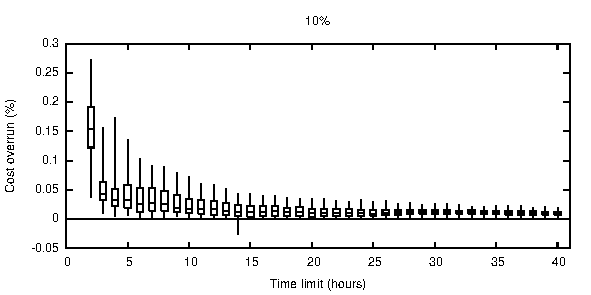
\includegraphics[width=0.7\columnwidth]{BagOfTasks/tolerance-extended-10-2-cost-relative}  
     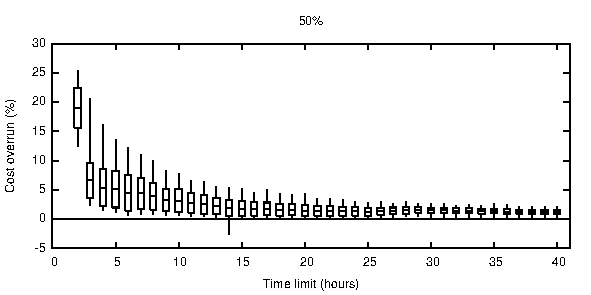
\includegraphics[width=0.7\columnwidth]{BagOfTasks/tolerance-extended-50-2-cost-relative}  
 	   \caption{Impact of runtime variation on cost overrun as a function of deadline. 
 	   Results obtained for random variation of task runtime in the range from $-10\%$ to $+10\%$ (top)
 	   and from $-50\%$ to $+50\%$ (bottom). }
 	   \label{fig:bot:dynamic-cost}
  \end{figure} 
  
  Fig.~\ref{fig:bot:dynamic-cost} shows the cost overrun with 10\% and 50\%  of runtime
  variation range.  The box-plots for each deadline represent averaged
  results for the data sizes from 0 to 256 MiB as in
  Fig.~\ref{fig:bot:sensitivity-surface}, with box boundaries at quartiles
  and whiskers at maximum and minimum values. We observe that the highest
  overruns are for the shortest deadlines, which results from the fact that
  when each VM instance runs only for a few hours, then the additional hour
  will incur relatively high additional cost. On the other hand, for longer
  deadlines the cost of additional VM-hour becomes less significant. We also
  observe that the aggregated impact of positive and negative variations in
  task execution time may cancel to nearly $0$ and in some cases the cost
  overrun may be negative.

  \begin{figure}[tb]
    \centering
    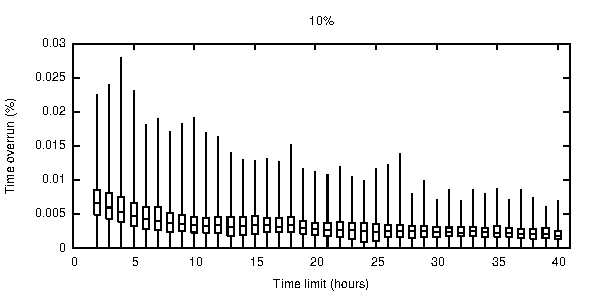
\includegraphics[width=0.7\columnwidth]{BagOfTasks/tolerance-extended-10-2-overrun-relative}       
    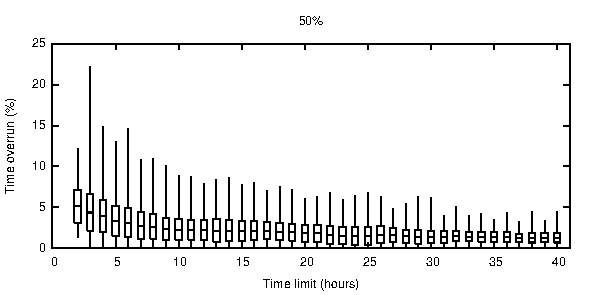
\includegraphics[width=0.7\columnwidth]{BagOfTasks/tolerance-extended-50-2-overrun-relative}  
    \caption{Impact of runtime variation on deadline overrun as a function of deadline. 
    Results obtained for random variation of task runtime in the range from $ -10\%$ to $10\%$ (top)
    and from $-50\%$ to $+50\%$ (bottom). }
    \label{fig:bot:dynamic-time}
  \end{figure} 

  In a similar way Fig.~\ref{fig:bot:dynamic-time} shows the deadline overrun in
  the presence of runtime variations. We can observe that the deadline overrun
  is much smaller than cost overrun. This means that the actual finish time of
  all tasks is not significantly affected by the runtime variation, due to the
  cancellation effect. We observe that even for high variations in the range
  from $-50\%$ to $50\%$ the actual runtime rarely exceeds the deadline by
  more than 10\%. This overrun can be thus easily compensated by solving the
  optimization problem with a respectively shorter deadline giving a safety
  margin in the case of expected high variations of actual task runtimes. Similar estimation is also possible in the case when the application consists of many tasks of similar size which distribution in known in advance. 
	


\section{Summary}

  In this chapter we discussed bag of tasks applications model and cloud infrastructure characteristics. This led us to formulating AMPL model for optimizing cost of running bag of tasks applications. The model was later evaluated in terms of optimization runtime and sensitivity. The results show that the total cost grows slowly for long deadlines, since   it is possible to use free resources from a private cloud. However, for short deadlines it is necessary to use the instances from public clouds, starting from the ones with best price/performance ratio. The shorter the deadlines, the more costly instance types have to be added, thus the cost grows more rapidly. Moreover, our results can be also useful for multi-objective optimization. In such a case, it would be possible to run the optimization algorithm in a certain neighborhood of the desired deadline and select the best solution using a specified cost/time trade-off. Alternatively, multiple solutions as in Fig.~\ref{fig:bot:large-finite},~\ref{fig:bot:sensitivity-surface}~or~\ref{fig:bot:cost_vs_data_size} may be corollary acceptable solution.

} % Command scope
